\documentclass[hyphens]{beamer}

\usepackage[utf8]{inputenc}
\usepackage[ngerman]{babel}

\usepackage{array}
\usepackage{tabularx}
\newcolumntype{Z}{>{\centering\let\newline\\\arraybackslash\hspace{0pt}}p{0.65\textwidth}}

\usepackage{amssymb}
\usepackage{pifont}
\newcommand{\xmark}{\ding{55}}

\usetheme[progressbar=frametitle,block=fill]{metropolis}

\setbeamertemplate{section in toc}[sections numbered]
\setbeamertemplate{subsection in toc}[subsections numbered]

\defbeamertemplate{subsubsection in toc}{subsubsections numbered}
{\leavevmode\leftskip=3em%
 \rlap{\hskip-3em\inserttocsectionnumber.\inserttocsubsectionnumber.\inserttocsubsubsectionnumber}%
 \inserttocsubsubsection\par}

\setbeamertemplate{subsubsection in toc}[subsubsections numbered]

\begin{document}
  \title[Gerät zur Schlaganfall-Rehabilitation]{Entwicklung eines Gamification-basierten Biofeedback-Unterstützungs- und Motivationsgeräts zur Rehabilitation von Schlaganfall-Patienten \\ \small{- Themenverteidigung -}}
  \author[Lukas Rost]{Lukas Rost  \\ \and \textsc{Fachbetreuer:} Johannes Süpke \and \textsc{Außenbetreuer:} Hannes Weichel}
  \institute[ASGspez]{Spezialschulteil des staatlichen Gymnasiums "'Albert Schweitzer"' Erfurt}
  \date{22. September 2017} 
  
 \begin{frame}
 \titlepage
 \end{frame}
 
  \begin{frame}
  \begin{figure}
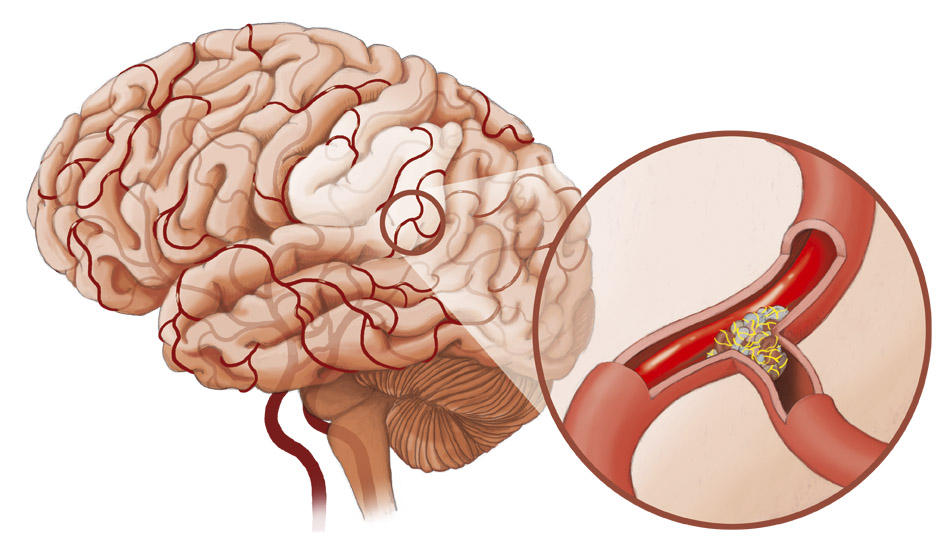
\includegraphics[scale=0.3]{pics/einleit2.jpg}
\end{figure}
 \end{frame}
 
 \begin{frame}
 \begin{figure}
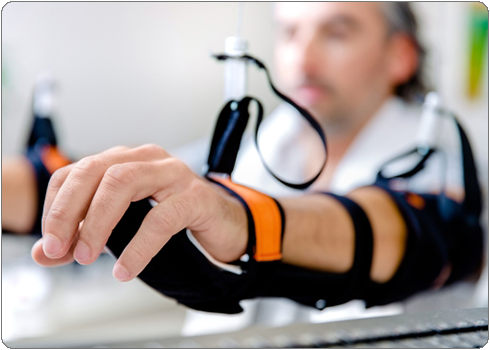
\includegraphics[scale=0.6]{pics/einleit1.png}
\end{figure}
 \end{frame}
 
 \begin{frame}
 \titlepage
 \end{frame}
 
 \begin{frame}{Gliederung}
 \tableofcontents
 \end{frame}
 
 \section{Zielstellung}
 \begin{frame}{Zielstellung}
 \begin{columns}[T]

\begin{column}{0.34\textwidth}
\begin{figure}
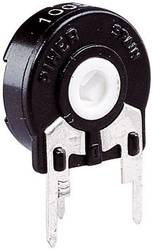
\includegraphics[width=0.7\textwidth]{pics/potentiometer-trimmer.jpg}
\end{figure}
\end{column}
\pause

\begin{column}{0.33\textwidth}
 ~ \\ ~ \\  ~ \\
\begin{figure}
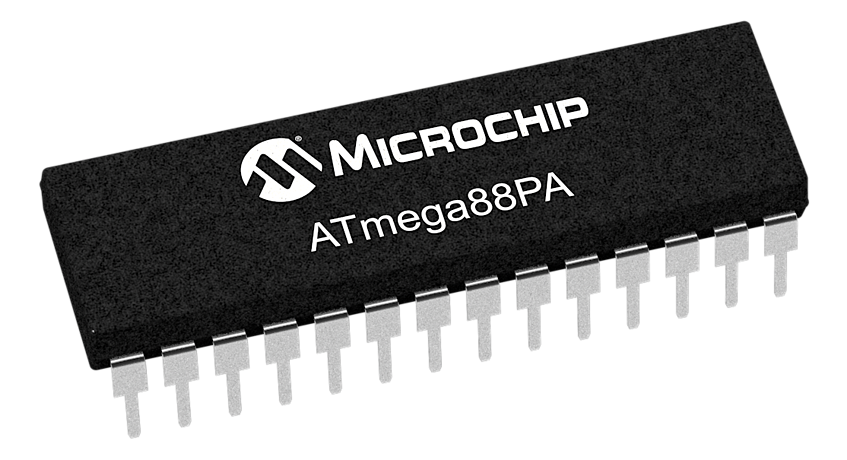
\includegraphics[width=\textwidth]{pics/ATmega88PA.png}
\end{figure}
\end{column}
\pause

\begin{column}{0.33\textwidth}
\begin{figure}
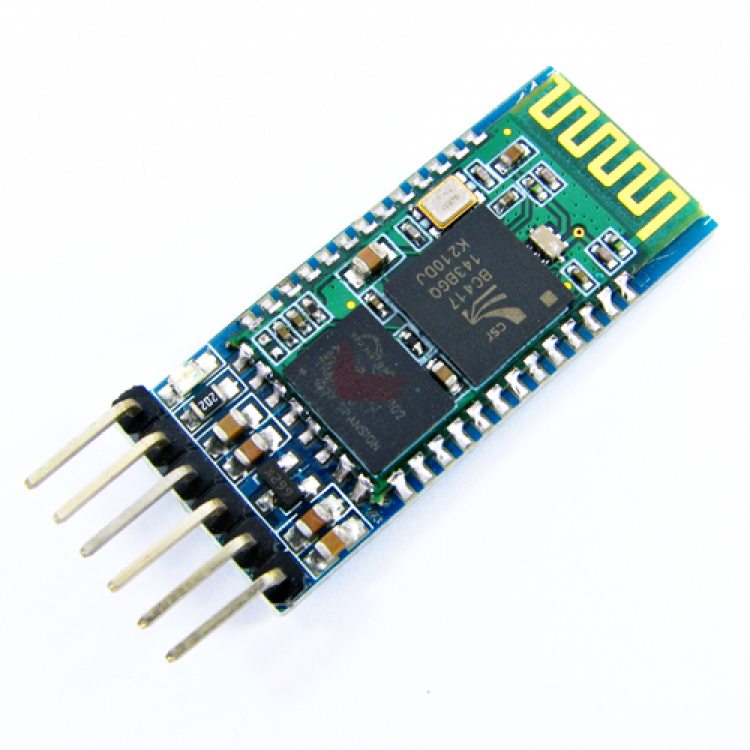
\includegraphics[width=\textwidth]{pics/HC05.png}
\end{figure}
\end{column}
\end{columns}
 \end{frame}
 
  \begin{frame}{Zielstellung}
 \begin{columns}[T]

\begin{column}{0.34\textwidth}
\begin{figure}

\includegraphics[width=\textwidth]{pics/android-logo.jpg}
\end{figure}
\end{column}
\pause

\begin{column}{0.33\textwidth}
\begin{figure}

\includegraphics[width=\textwidth]{pics/Google-Fit-Icon.png}
\end{figure}
\end{column}
\pause

\begin{column}{0.33\textwidth}
\begin{figure}

\includegraphics[width=\textwidth]{pics/playn-logo.png}
\end{figure}
\end{column}
\end{columns}
 \end{frame}
 
 \subsection{Gliederung der Arbeit}
 \begin{frame}{Gliederung der Arbeit}
 \begin{figure}
\centering 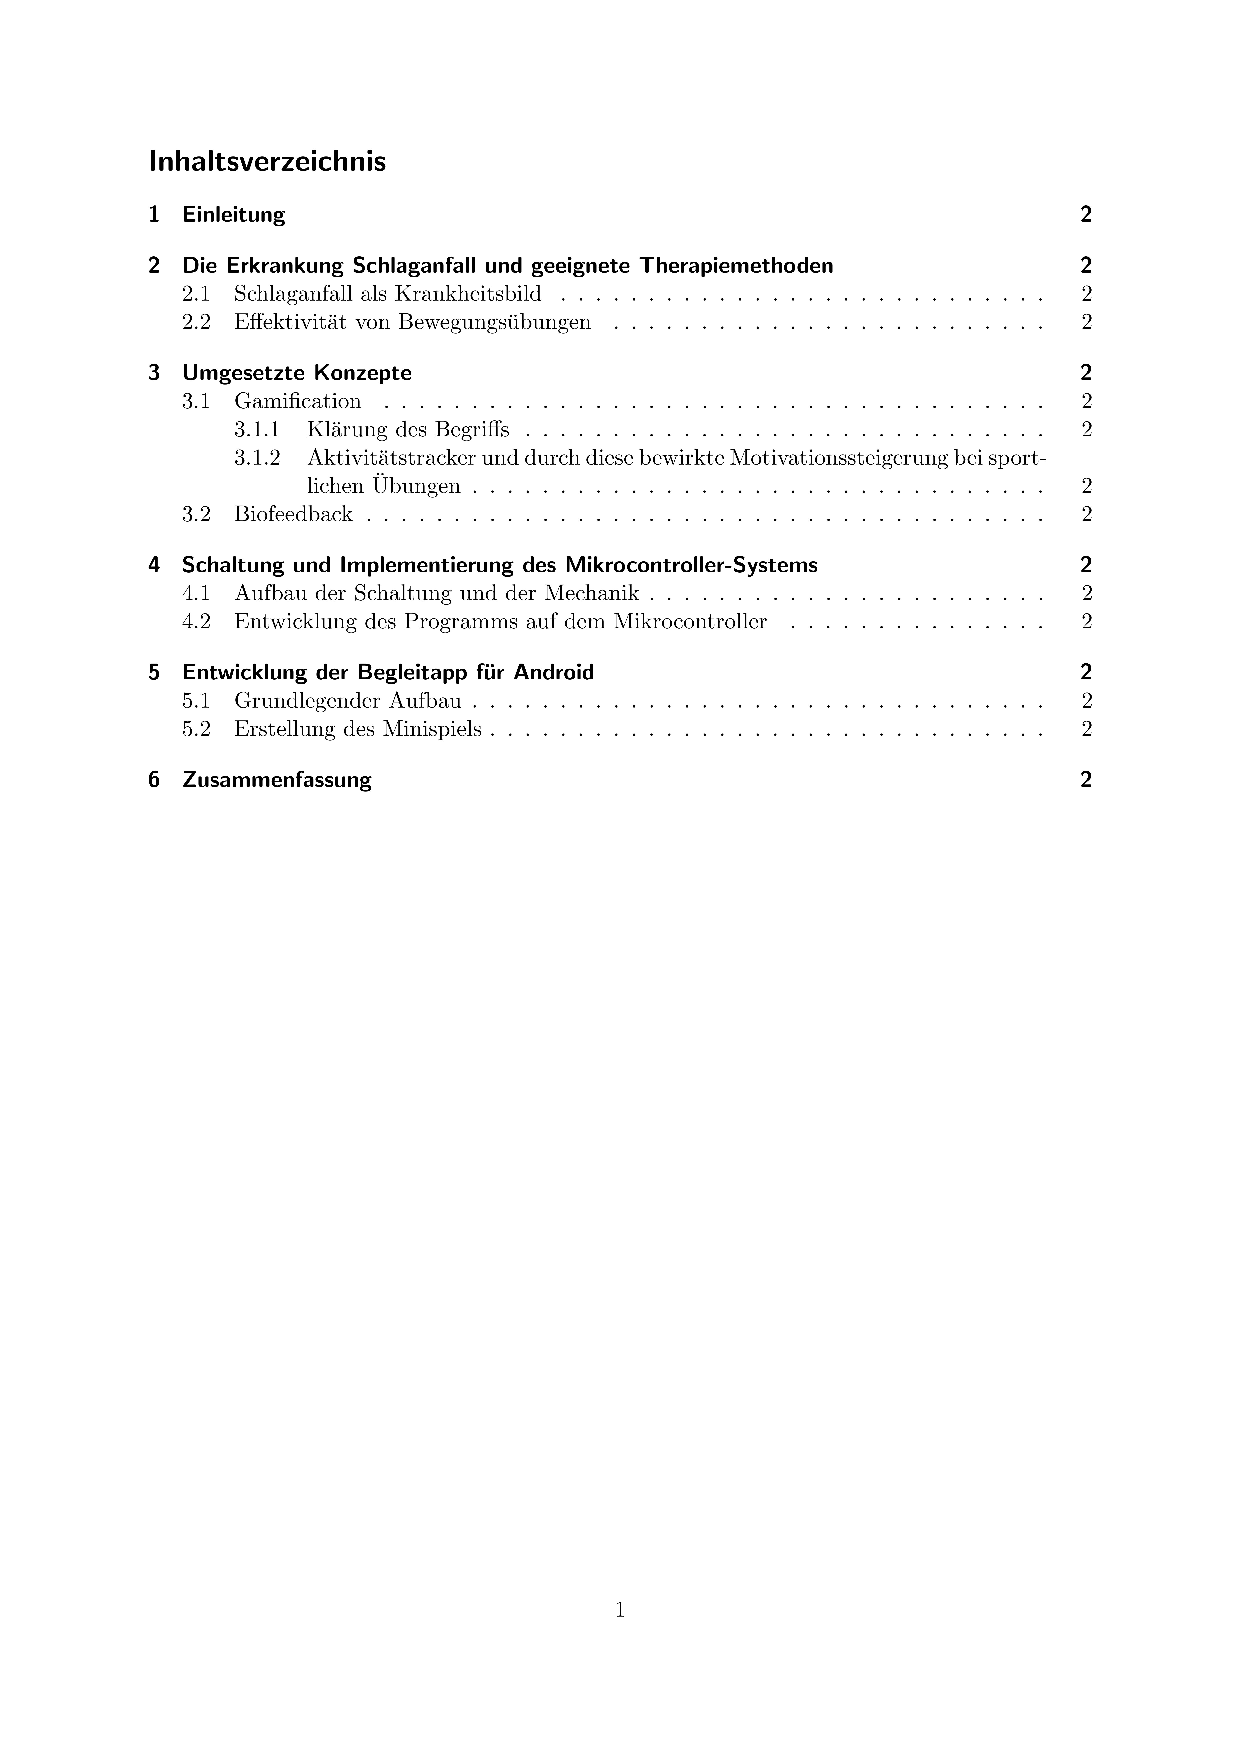
\includegraphics[width=\textwidth]{pics/gliederung.pdf}
\end{figure}
 \end{frame}
 
 \section{Einordnung und Abgrenzung}
 \begin{frame}{Einordnung und Abgrenzung}
 \begin{itemize}[<+->]
 \item Was die Arbeit \emph{nicht} leisten soll
 		\begin{itemize}
 		\item[-] \emph{keine} ausführliche Behandlung der Erkrankung Schlaganfall
 		\item[-] \emph{keine} ausführliche Abhandlung aller möglichen Therapiemethoden
 		\item[-] \emph{keine} Fitness-App für normale Sportarten
 		\item[-] \emph{kein} Anspruch auf spätere Serienfertigbarkeit
 		\end{itemize}
 \end{itemize}

 \end{frame}
 
 \section{Methodisches Vorgehen}
 \begin{frame}{Methodisches Vorgehen}
 \begin{itemize}[<+->]
 \item Literaturstudium zu:
 		\begin{itemize}
 		\item[-] ATmega-Mikrocontrollern und deren Programmierung
 		\item[-] App-Programmierung für Android
 		\item[-] Gamification und Biofeedback
 		\item[-] Erkrankung Schlaganfall
 		\item[-] Effektivität von Schlaganfall-Bewegungsübungen
 		\item[-] Motivationssteigerung bei Aktivitätstrackern
 		\end{itemize}
 \item Entwicklung von:
 		\begin{itemize}
 		\item[-] Programm und Schaltung für den Mikrocontroller
 		\item[-] Begleitapp für Android
 		\end{itemize}
 \end{itemize}
 \end{frame}
 
 \subsection{Zeitplan}
 \begin{frame}{Zeitplan}
 \begin{flushleft}
 \begin{table}
 \begin{small}
 \begin{tabularx}{\columnwidth}{p{0.35\textwidth}|Z}
 \hline
 Zeitraum & Aufgabe \\ \hline
 September 2017 bis November 2017 & Literaturstudium zur Programmierung des Mikrocontrollers und geeigneten Bewegungsübungen \\ \hline
 Dezember 2017 bis Februar 2018 & Programmierung des Mikrocontrollers \\ \hline
 März 2018 bis April 2018 & Bau der Mechanik für das Gerät \\ \hline
 Mai 2018 bis Juni 2018 & Literaturstudium zur Entwicklung der Android-App -$>$ Konzept \\ \hline
 27. Juni 2018 & Zwischenstandsverteidigung \\ \hline
 Juli 2018 bis August 2018 & Entwicklung der App im Grundzustand \\ \hline
 September 2018 & Entwicklung des Minispiels \\ \hline
 Oktober 2018 bis Dezember 2018 & Literaturstudium zum theoretischen Teil der Arbeit und Fertigstellung dieser -$>$ Abgabe \\ \hline
 Januar 2019 bis März 2019 & Vorbereitung auf das Kolloquium, evtl. Praxistest -$>$ Kolloquium \\ \hline
 \end{tabularx}
 \end{small}
 \end{table}
 \end{flushleft}
 \end{frame}

 \begin{frame}{Bildquellen}
 \begin{itemize}
 \tiny{\item \url{http://www.lahsit-schlaganfall-reha.de/images/slider/lahsit-banner-3.png}}
 \item \tiny{\url{http://www.bayern-schlaganfall.de/fileadmin/_migrated/pics/weisser_Infarkt_02.jpg}}
 \item \tiny{\url{https://asset.conrad.com/media10/isa/160267/c1/-/de/431176_BB_00_FB/trimmer-linear-025-w-500-k-250-270-piher-pt-15-lh-500k-1-st.jpg?x=250&y=250}}
 \item \tiny{\url{http://www.microchip.com/_images/ics/medium-ATmega88PA-SPDIP-28.png}}
 \item \tiny{\url{http://bdspeedytech.com/image/cache/catalog/Bluetooth-750x750.png}}
 \item \tiny{\url{https://image.freepik.com/vektoren-kostenlos/android-boot-logo_634639.jpg}}
 \item \tiny{\url{http://www.playn-2011.appspot.com/slides/images/playn-logo.png}}
 \item \tiny{\url{https://upload.wikimedia.org/wikipedia/commons/6/60/Google-Fit-Icon.png}}
 \end{itemize}
 \end{frame}
 
 \begin{frame}
 \titlepage
 \end{frame}
  
\end{document}
